%%
%% This is file `elsarticle-template-num.tex',
%% generated with the docstrip utility.
%%
%% The original source files were:
%%
%% elsarticle.dtx  (with options: `numtemplate')
%% 
%% Copyright 2007, 2008 Elsevier Ltd.
%% 
%% This file is part of the 'Elsarticle Bundle'.
%% -------------------------------------------
%% 
%% It may be distributed under the conditions of the LaTeX Project Public
%% License, either version 1.2 of this license or (at your option) any
%% later version.  The latest version of this license is in
%%    http://www.latex-project.org/lppl.txt
%% and version 1.2 or later is part of all distributions of LaTeX
%% version 1999/12/01 or later.
%% 
%% The list of all files belonging to the 'Elsarticle Bundle' is
%% given in the file `manifest.txt'.
%% 

%% Template article for Elsevier's document class `elsarticle'
%% with numbered style bibliographic references
%% SP 2008/03/01

%\documentclass[preprint,12pt]{elsarticle}
\documentclass[preprint,10pt]{elsarticle}
%\documentclass[final,3p,times]{elsarticle} 

%% Use the option review to obtain double line spacing
%% \documentclass[authoryear,preprint,review,12pt]{elsarticle}

%% Use the options 1p,twocolumn; 3p; 3p,twocolumn; 5p; or 5p,twocolumn
%% for a journal layout:
%% \documentclass[final,1p,times]{elsarticle}
%% \documentclass[final,1p,times,twocolumn]{elsarticle}
%% \documentclass[final,3p,times]{elsarticle}
%% \documentclass[final,3p,times,twocolumn]{elsarticle}
%% \documentclass[final,5p,times]{elsarticle}
%% \documentclass[final,5p,times,twocolumn]{elsarticle}


\usepackage{array}
\usepackage{color}
\usepackage{graphicx}
\usepackage{float} % utiliser H pour forcer a mettre l'image ou on veut
\usepackage{mathbbol} % permet d'avoir le vrai symbol pour les reels grace a mathbb
\usepackage{stmaryrd} % permet d'utiliser \llbrackedt et \rrbracket : double crochet
\usepackage{subfigure}
\usepackage{appendix}

%% The amssymb package provides various useful mathematical symbols 
%% The amsthm package provides extended theorem environments
\usepackage{amssymb}
\usepackage{amsmath}
% more math
\usepackage{amsfonts}
\usepackage{amssymb}
\usepackage{amstext}
\usepackage{amsbsy}


%% The lineno packages adds line numbers. Start line numbering with
%% \begin{linenumbers}, end it with \end{linenumbers}. Or switch it on
%% for the whole article with \linenumbers.
\usepackage{lineno}

\journal{TTSP}

\newcommand\bn{\boldsymbol{\nabla}}
\newcommand\bo{\boldsymbol{\Omega}}
\newcommand\br{\mathbf{r}}
\newcommand\la{\left\langle}
\newcommand\ra{\right\rangle}
\newcommand\bs{\boldsymbol}
\newcommand\red{\textcolor{red}}
\newcommand\ldb{\{\!\!\{}
\newcommand\rdb{\}\!\!\}}
\newcommand\llb{\llbracket}
\newcommand\rrb{\rrbracket}

\renewcommand{\(}{\left(}
\renewcommand{\)}{\right)}
\renewcommand{\[}{\left[}
\renewcommand{\]}{\right]}

\usepackage{setspace}
\newcommand{\tr}[1]{\textcolor{red}{#1}}
\newcommand{\tri}[1]{\textcolor{red}{{\it #1}}}

%%%%%%%%%%%%%%%%%%%%%%%%%%%%%%%%%%%%%%%%%%%%%%%%%%%%%%%%%%%%%%%%%%%%
% operators
\renewcommand{\div}{\vec{\nabla}\! \cdot \!}
\newcommand{\grad}{\vec{\nabla}}
% latex shortcuts
\newcommand{\bea}{\begin{eqnarray}}
\newcommand{\eea}{\end{eqnarray}}
\newcommand{\be}{\begin{equation}}
\newcommand{\ee}{\end{equation}}
\newcommand{\bal}{\begin{align}}
\newcommand{\eali}{\end{align}}
\newcommand{\bi}{\begin{itemize}}
\newcommand{\ei}{\end{itemize}}
\newcommand{\ben}{\begin{enumerate}}
\newcommand{\een}{\end{enumerate}}
% DGFEM commands
\newcommand{\jmp}[1]{[\![#1]\!]}                     % jump
\newcommand{\mvl}[1]{\{\!\!\{#1\}\!\!\}}             % mean value
\newcommand{\keff}{\ensuremath{k_{\textit{eff}}}\xspace}
% shortcut for domain notation
\newcommand{\D}{\mathcal{D}}
\newcommand{\J}{\mathcal{J}}
\newcommand{\I}{\mathcal{I}}
% vector shortcuts
\newcommand{\vo}{\vec{\Omega}}
\newcommand{\vr}{\vec{r}}
\newcommand{\vn}{\vec{n}}
\newcommand{\vnk}{\vec{\mathbf{n}}}
\newcommand{\vj}{\vec{J}}
% extra space
\newcommand{\qq}{\quad\quad}
% common reference commands
\newcommand{\eqt}[1]{Eq.~(\ref{#1})}                     % equation
\newcommand{\fig}[1]{Fig.~\ref{#1}}                      % figure
\newcommand{\tbl}[1]{Table~\ref{#1}}                     % table
\newcommand{\sct}[1]{Section~\ref{#1}}                   % section

\newcommand{\ud}{\,\mathrm{d}}
\newcommand{\mt}[1]{\marginpar{{\singlespacing \textcolor{red}{{\tiny #1}}}}}
\newcommand{\Half}{\text{\it Half\,}}

%%%%%%%%%%%%%%%%%%%%%%%%%%%%%%%%%%%%%%%%%%%%%%%%%%%%%%%%%%%%%%%%%%%%%
%
%   BEGIN DOCUMENT
%
%%%%%%%%%%%%%%%%%%%%%%%%%%%%%%%%%%%%%%%%%%%%%%%%%%%%%%%%%%%%%%%%%%%%%
\begin{document}

%%%%%%%%%%%%%%%%%%%%%%%%%%%%%%%%%%%%%%%%%%%%%%%%%%%%%%%%%%%%%%%%%%%%
\begin{frontmatter}

%% Title, authors and addresses

%% use the tnoteref command within \title for footnotes;
%% use the tnotetext command for theassociated footnote;
%% use the fnref command within \author or \address for footnotes;
%% use the fntext command for theassociated footnote;
%% use the corref command within \author for corresponding author footnotes;
%% use the cortext command for theassociated footnote;
%% use the ead command for the email address,
%% and the form \ead[url] for the home page:
%\title{Title\tnoteref{label1}}
%% \tnotetext[label1]{}
%% \author{Name\corref{cor1}\fnref{label2}}
%% \ead{email address}
%% \ead[url]{home page}
%% \fntext[label2]{}
%% \cortext[cor1]{}
%% \address{Address\fnref{label3}}
%% \fntext[label3]{}

%-------------------------
%-------------------------
\title{Angular Multigrid Preconditioner for Krylov-based Solution Techniques
applied to the $S_n$ Equations with Highly Forward-Peaked Scattering}
\author{abc} 

\begin{abstract}
It is well known that diffusion synthetic acceleration (DSA) methods for the
$S_n$ equations become ineffective in the Fokker-Planck forward-peaked
scattering limit. In response to this deficiency, Morel and Manteuffel
\cite{multigrid_1d} developed an angular multigrid method for the 1-D $S_n$
equations. This method is very effective, costing roughly twice as much as DSA
per source iteration, but yielding a maximum spectral radius of approximately
$0.6$ in the Fokker-Planck limit. Pautz, Adams, and Morel (PAM) later
generalized to 2-D \cite{multigrid_2d}, but it was found that the method was
unstable with sufficiently forward-peaked mappings between the angular grids.
The method was stabilized via a filtering technique based upon diffusion
operators, but this filtering also degraded the effectiveness of the overall
scheme. The spectral radius was not bounded away from unity in the
Fokker-Planck limit, although the method remained more effective than DSA. The
purpose of this paper is to recast the 2-D PAM angular multigrid method
without the filtering as an $S_n$ preconditioner and use it in conjunction
with the GMRES Krylov method. The approach ensures stability, and our
computational results demonstrate that it is also significantly more efficient
than an analogous DSA-preconditioned Krylov method.
\end{abstract}

%-------------------------
\begin{keyword}
aaa \sep
bbb.
\end{keyword}
%-------------------------
\end{frontmatter}
%-------------------------

%%%%%%%%%%%%%%%%%%%%%%%%%%%%%%%%%%%%%%%%%%%%%%%%%%%%%%%%%%%%%%%%%%%%
\linenumbers
\doublespacing

%%%%%%%%%%%%%%%%%%%%%%%%%%%%%%%%%%%%%%%%%%%%%%%%%%%%%%%%%%%%%%%%%%%%
%%%%%%%%%%%%%%%%%%%%%%%%%%%%%%%%%%%%%%%%%%%%%%%%%%%%%%%%%%%%%%%%%%%%
\section{Introduction}
%%%%%%%%%%%%%%%%%%%%%%%%%%%%%%%%%%%%%%%%%%%%%%%%%%%%%%%%%%%%%%%%%%%%
%%%%%%%%%%%%%%%%%%%%%%%%%%%%%%%%%%%%%%%%%%%%%%%%%%%%%%%%%%%%%%%%%%%%
The discrete ordinates method has been shown to be quite accurate for electron
and coupled electron-photon transport \cite{morel_81,accuracy_1,accuracy_2}, 
which is required in the
development of radiation therapy protocols, satellite electronics shielding,
flash x-ray machine design, and a wide variety of other applications. Charged
particles interact through Coulomb interactions with the background medium.
Such interactions predominately result in extremely small changes in particle
direction and energy. Such interactions are well characterized by the
Fokker-Planck limit of the transport equation \cite{fp_limit,morel_96}. In this limit,
the directional and energy changes are decoupled with former modeled by the
continuous scattering operator and the latter modeled by the
continuous-slowing-down operator. In this paper, we consider the
discrete-ordinate ($S_n$) angular discretization of the transport equation
with a focus upon iterative solution methods for problems with highly
forward-peaked scattering characteristic of the Fokker-Planck limit. In this
limit, the mean-free-path and the directional change per scattering
interaction goes to zero while the momentum transfer (also called the
transport-corrected scattering cross section) remains fixed.

When the scattering is highly forward-peaked, solving the $S_n$ transport
equation can be challenging due to the slow convergence of standard iterative
algorithm, such as Source Iteration (SI). To speed up iterative convergence,
acceleration schemes such as Diffusion Synthetic Acceleration (DSA) are used.
With isotropic or weakly anisotropic scattering, DSA is generally highly
effective \cite{adams}, but it becomes completely ineffective in the
Fokker-Planck limit \cite{multigrid_1d}.

To address this deficiency, a 1-D angular multigrid method for the $S_n$
equations was developed by Morel and Manteuffel (MM) \cite{multigrid_1d}. This
method was extremely efficient yielding a maximum spectral radius for a model
a model infinite-medium problem of approximately 0.6 at a cost of
approximatively twice that of DSA. This maximum spectral radius is approached
in the Fokker-Planck limit. In this same limit, the spectral radius of DSA
approaches 1.

Pautz, Adams, and Morel (PAM) \cite{multigrid_2d} generalized the MM method to
2-D, but it was found to be stable only for weakly forward-peaked scattering.
The instability arose from high-frequency spatial error amplification that
occurred in the transfer of error estimates between angular grids (a sequence
of different $S_n$ orders). Stabilization was achieved by filtering the error
estimates via diffusion operators. However, this filtering was expensive and
significantly degraded the effectiveness of the method such that the spectral
radius approaches $1$ in the Fokker-Planck limit.

The purpose of the present work is to investigate recasting of the PAM method
with no filtering (PAMNF) as a preconditioner and using it in conjunction with
the GMRES Krylov method. In this form, stability of the iteration scheme is
guaranteed. We compute the eigenvalues of preconditioned system for a model
problem and compare the spectrum with those of preconditioners based upon
sweep and DSA. It is found that relative to these preconditioners,
PAMNF preconditioning moves the eigenvalues away from zero while leaving them
constrained to a reasonably small portion of the complex plane. These are
desirable properties for a preconditioner. We also compare the convergence
rates and efficiency of these preconditioners for various test problems with
forward-peaked scattering. We find that PAMNF preconditioning
is significantly more efficient than both sweep and DSA
preconditioning, and become increasingly so as the Fokker-Planck limit is
approached. However, the number of iterations required for convergence
nonetheless increases as this limit is approached. Thus, optimal multigrid
performance is not achieved. In spite of this fact, the PAMNF-preconditioned
Krylov method achieves good efficiency without the costly filtering associated
with the original PAM fixed-point iteration scheme, appears to be more
effective than other existing algorithms for solving the $S_n$ equations with
highly forward-peaked scattering.

The remainder of this paper this paper is organized as follows. In
Sec.(\ref{sec:anisotropy}), we
discuss the anisotropic scattering treatment used in $S_n$ calculations and
certain special requirements associated with highly forward-peaked scattering.
In particular, we discuss Legendre scattering source expansions, the extended
transport correction, and the need for Galerkin quadrature. In
Sec.(\ref{sec:iterative_scheme}), we
discuss the source iteration, DSA, and PAMNF iteration schemes. In
Sec.(\ref{sec:preconditioner}), we
discuss the simple manner in which any fixed-point iteration scheme can be
recast as preconditioner for use in conjunction with a Krylov solver. In
Sec.(\ref{sec:spectrum}),
we compare the eigenvalue spectra of the sweep, DSA, and PAMNF
preconditioners. In Sec.(\ref{sec:results}), we present computational comparisons of the
preconditioners, and in Sec.(\ref{sec:conclusions}), we give our conclusions. Finally, we give
detailed operator representations for the DSA, and PAMNF
preconditioners in the Appendix.

%-------------------------
%%%%%%%%%%%%%%%%%%%%%%%%%%%%%%%%%%%%%%%%%%%%%%%%%%%%%%%%%%%%%%%%%%%%%%%%%%%%%%%%%%%%
%%%%%%%%%%%%%%%%%%%%%%%%%%%%%%%%%%%%%%%%%%%%%%%%%%%%%%%%%%%%%%%%%%%%%%%%%%%%%%%%%%%%
\section{Anisotropic scattering} \label{sec:anisotropy}
%%%%%%%%%%%%%%%%%%%%%%%%%%%%%%%%%%%%%%%%%%%%%%%%%%%%%%%%%%%%%%%%%%%%%%%%%%%%%%%%%%%%
%%%%%%%%%%%%%%%%%%%%%%%%%%%%%%%%%%%%%%%%%%%%%%%%%%%%%%%%%%%%%%%%%%%%%%%%%%%%%%%%%%%%

Charged particles transport can be described by the Boltzmann equation
\cite{graal}, discretized in energy using the standard multigroup method
and in angle using the discrete ordinate method ($S_n$)
\mt{Reuss, really?}\cite{reuss}. For the purpose of this paper, we restrict ourselves to the one-group $S_n$ equation,
given below in \eqt{eq:1-g_sn}; however, the techniques described apply straightforwardly to the multigroup equations:
%
\begin{equation}
\bo_d \cdot \bn \Psi_d(\br) + \Sigma_{t}(\br) \Psi_d(\br) = 
\sum_{l=0}^L\sum_{m=-l}^l \frac{2l+1}{4\pi}\Sigma_{s,l}
\Phi_{l,m}(\br)Y_l^m(\bo_d) + Q_d(\br) ,
\label{eq:1-g_sn}
\end{equation}
%
where $\br$ is the position in domain $\mathcal{D}$, $\bo_d=(\mu_d,\varphi_d)$, 
$\mu_d$ is the cosine of the directional polar angle,
$\varphi_d$ is the directional azimuthal angle, $\Psi_d$ is
the angular flux in direction $d$, $Q_d$ is a volumetric source, $\Sigma_{t}(\br)$ is the total 
macroscopic cross section, $\Sigma_{s,l}$ is the Legendre moment of 
degree $l$ of the scattering cross section $\Sigma_s$, and $\Phi_{l,m}(\br,E)= \int_{4\pi}\Psi(\br,\bo,E)A_l^{m}(\bo)\ d\bo
\approx \sum_{d=1} w_d \Psi(\br,\bo_d,E)Y_l^{m}(\bo_d)$ with  $A_l^m$ the 
real spherical harmonics.
%
Boundary conditions need to be applied to \eqt{eq:1-g_sn} to close the system; the most
commonly employed is the incoming flux boundary condition:
%
\begin{equation}
\Psi(\br,\bo,E) = g(\br,\bo,E)\textrm{ for }\bo\cdot\bs{n}<0\textrm{ and
}\br\in \partial \mathcal{D},
\label{eq:boundary}
\end{equation} 
%
where $\partial \mathcal{D}$ is the boundary of the domain $\mathcal{D}$. If $g=0$, \eqt{eq:boundary}
yields vacuum boundary conditions.\\
When solving a mutligroup coupled electron-photon problem, the cross sections employed are typically generated using
the CEPXS code \cite{cepxs}. For one-group models of highly-forward peaked scattering, Fokker-Planck cross sections 
are typically used \hbox{\cite{multigrid_1d,multigrid_2d,morel_81,morel_96} :}
%
\begin{equation}
\Sigma_{s,l}=\frac{\alpha}{2} (L(L+1)-l(l+1))\ \ l=0,\hdots,L ,
\end{equation}
%
where $\alpha$ is the restricted momentum transfer.
These cross sections are a Legendre-moment representation of the
continuous-scattering operator \cite{morel_96} :
%
\begin{equation}
\Gamma = \frac{\alpha}{2} \(\frac{\partial }{\partial \mu}\((1-\mu^2)\frac{\partial
}{\partial \mu}\)+\frac{1}{1-\mu^2}\frac{\partial^2}{\partial \varphi}\)
\end{equation}
%
This operator, present in the Boltzmann-Fokker-Planck equation, is used to describe
charged-particle transport \cite{morel_81,morel_96} and is the asymptotic 
limit of the  Boltzmann scattering operator when the $\Sigma_s$ becomes 
unbounded and the average cosine angle $\bar{\mu}_0$ tends towards unity in 
such a manner that $\alpha = \Sigma_s(1-\bar{\mu}_0)$ remains constant.\\

One of key features of angular multigrid method is that transport sweeps
can strongly damp the high frequency error modes (upper half of the flux moments) with the
use an ``optimal'' transport correction \cite{multigrid_1d}. 
This ``optimal'' transport correction is a variant of the
more known extended transport correction \cite{lathrop,morel_79}. The transport
correction is a modification of the cross-section moments that changes the effect
of the transport sweeps and consists in subtracting a Dirac value from the cross
sections. 
%The ``optimal'' transport correction increases the efficiency of the sweeps to damp the high frequency error modes. 

Subtracting a Dirac distribution from the cross sections will not change the result of the $S_n$ 
calculations if the Dirac distribution is integrated exactly. Therefore, a Galerkin quadrature
will have to be used \cite{graal}. Galerkin quadratures require that the discrete-to-moment matrix ($D$)
and the moment-to-discrete matrix ($M$) satisfy
%
\begin{equation}
MD = I,
\end{equation}
%
where $I$ is the identity matrix. $M$ maps a vector of flux moments to a 
vector of discrete angular flux values and $D$ maps a vector of discrete 
angular flux values to a vector of flux moments. It is easy to note that Galerkin quadratures exactly 
integrate a Dirac distribution. For example, assume that:
%
\begin{equation}
\Sigma_s(\mu) = a\delta(\mu-1).
\end{equation}
%
Then, the (exact) scattering operator is given by :
%
\begin{equation}
R= \int_{4\pi} \Sigma_s(\bo\cdot\bo')\Psi(\bo')d\bo'
=\int_{-1}^1 a\delta(\mu-1)\Psi(\mu)d\mu
=a\Psi
\end{equation}
%
In the discretized $S_n$ equations, the scattering operator is
%
\begin{equation}
\bs{R} = M\Sigma D \bs{\Psi},
\end{equation}
%
where $\bs{R}$ is the vector containing the source moments, $\Sigma$ is the scattering
matrix containing the moments of the scattering cross sections on its
diagonal, and $\bs{\Psi}$ is the vector containing the angular flux for all directions.
The cross-section matrix for a Dirac function is the identity matrix and,
therefore, the discretized scattering term, when a Galerkin quadrature is used, is given by :
%
\begin{equation}
\bs{R} = M\Sigma D \bs{\Psi} = M aI D \bs{\Psi} =a\bs{\Psi}
\end{equation}
%

\eqt{eq:1-g_sn} is also discretized in space. The solution techniques proposed
in this paper for highly forward peaked scattering are not restricted to a 
particular spatial discretization. The results presented here have been obtained 
using bilinear discontinuous finite elements in two dimensional space \cite{dgfem}.
Upon space anf angle discretizations, \eqt{eq:1-g_sn} can be re-cast using operator notation as follows:
%
\begin{equation}
L \bs{\Psi} = M\Sigma D \bs{\Psi} + \bs{Q},
\label{eq:operator}
\end{equation}
%
where $\bs{\Psi}$ is a vector containing all the $\Psi_d$, $\bs{Q}$ is a
vector containing all the $Q_d$, $\Sigma$ is a diagonal matrix with 
$\Sigma_{s,l}$ values as diagonal entries, $M$ is the moment-to-discrete
matrix $(\bs{\Psi} = M\bs{\Phi})$, $D$ is the discrete-to-moments matrix
$(\Phi=D\Psi)$ (the specific spherical moment entries are dictated by (1) the choice of 
the angular quadrature and (2) the dimensionality of the problem) and 
$L = \bo\cdot\grad + \Sigma_t$ is the streaming + total interaction operator,
inverted direction by direction (transport sweeps). The inversion can be done
locally for each mesh cell for each discrete directional flux in the
quadrature.\\

%%%%%%%%%%%%%%%%%%%%%%%%%%%%%%%%%%%%%%%%%%%%%%%%%%%%%%%%%%%%%%%%%%%%%%%%%%%%%%%%%%%%
%%%%%%%%%%%%%%%%%%%%%%%%%%%%%%%%%%%%%%%%%%%%%%%%%%%%%%%%%%%%%%%%%%%%%%%%%%%%%%%%%%%%
\section{Iterative schemes for highly forward-peaked scattering} \label{sec:iterative_scheme}
%%%%%%%%%%%%%%%%%%%%%%%%%%%%%%%%%%%%%%%%%%%%%%%%%%%%%%%%%%%%%%%%%%%%%%%%%%%%%%%%%%%%
%%%%%%%%%%%%%%%%%%%%%%%%%%%%%%%%%%%%%%%%%%%%%%%%%%%%%%%%%%%%%%%%%%%%%%%%%%%%%%%%%%%%

%%%%%%%%%%%%%%%%%%%%%%%%%%%%%%%%%%%%%%%%%%%%%%%%%%%%%%%%%%%%%%%%%%%%%%%%%%%%%%%%%%%%
\subsection{Source Iteration and DSA}
%%%%%%%%%%%%%%%%%%%%%%%%%%%%%%%%%%%%%%%%%%%%%%%%%%%%%%%%%%%%%%%%%%%%%%%%%%%%%%%%%%%%

\eqt{eq:operator} can be solved using the Source Iteration (SI) method or a
Krylov method. The Source Iteration method at the $k^{th}$ iteration is given
by:
%
\begin{equation}
\bs{\Phi}^{(k+1)} = DL^{-1}M\Sigma \bs{\Phi}^{(k)} + DL^{-1}\bs{Q} .
\end{equation}
%
The spectral radius of SI can become arbitrary close to one when the
scattering ratio $c=\max\(\frac{\Sigma_{s,l}}{\Sigma_t}\)$ is close to one.
Since most physical forward-peaked scattering produces
$\Sigma_{s,0}>\Sigma_{s,1}>\hdots$, the flat modes are the ones which should
be accelerated. The Diffusion Synthetic Acceleration scheme \cite{adams} is
commonly used to accelerate this flat modes. The SI+DSA scheme is given by
%
a transport sweep
%\begin{subequations}
\begin{equation}
\bs{\Phi}^{(k+1/2)} = DL^{-1}M\Sigma\bs{\Phi}^{(k)} + DL^{-1}\bs{Q},
\end{equation}
%
followed by a diffusion synthetic acceleration
%
\begin{equation}
\delta\bs{\Phi}^{(k)} = \mathcal{T}_0^{-1} R_{n\rightarrow 0} 
\(\bs{\Phi}^{(k+1/2)}-\bs{\Phi}^{(k)}\) .
\end{equation}
%\end{subequations}
%
yielding the next iterate for the flux moments
%
\begin{equation}
\bs{\Phi}^{(k+1)} = \bs{\Phi}^{(k+1/2)} + P_{0/1 \rightarrow n} \delta 
\bs{\Phi}^{(k)} .
\end{equation}
%
Finally, we obtain:
%
\begin{multline}
\bs{\Phi}^{(k+1)} = \((I+P_{0/1\rightarrow n} \mathcal{T}_0^{-1} R_{n\rightarrow 0} )
DL^{-1}M\Sigma-P_{0/1\rightarrow n}\mathcal{T}_0^{-1} R_{n\rightarrow 0}\)
\bs{\Phi}^{(k)}\\ + (I+P_{0/1\rightarrow n}\mathcal{T}_0^{-1}
R_{n\rightarrow 0})DL^{-1} Q ,
\end{multline}
%
where $\mathcal{T}_0$ is the DSA operator, $R_{n\rightarrow 0}$ is the
restriction matrix of $\bs{\Phi}_{n}$ (all moments) to $\bs{\Phi}_0$ (only 0-th moment) and $P_{0/1 \rightarrow
n}$ is the projection matrix of $\bs{\Phi}_0$ or $\bs{\Phi}_1$, depending
whether only the zeroth or the zeroth and the first moment are accelerated, onto
$\bs{\Phi}_n$. When only the zeroth moment is accelerated, the scheme is always
stable and the spectral radius is
$\max\(\rho_{iso},\frac{\Sigma_{s,1}}{\Sigma_t}\)$ where $\rho_{iso}$ is the
spectral radius when the scattering is isotropic. When both the zeroth and the
first moment are accelerated, the scheme is not always stable. The spectral
radius is given by
$\max\(\rho_{iso},\frac{\Sigma_{s,1}}{\Sigma_t-\Sigma_{s,1}}\)$
\cite{multisweep}. For highly forward peaked scattering, accelerating the zeroth moment 
is ineffective, whereas accelerating both moments can clearly be unstable.

%%%%%%%%%%%%%%%%%%%%%%%%%%%%%%%%%%%%%%%%%%%%%%%%%%%%%%%%%%%%%%%%%%%%%%%%%%%%%%%%%%%%
\subsection{Review of Previous Angular Multigrid Work} 
%%%%%%%%%%%%%%%%%%%%%%%%%%%%%%%%%%%%%%%%%%%%%%%%%%%%%%%%%%%%%%%%%%%%%%%%%%%%%%%%%%%%

\subsubsection{One dimensional geometry}
%%%%%%%%%%%%%%%%%%%%%%%%%%%%%%%%%%%%%%%%%%%%%%%%%%%%%%%%%%%%%%%%%%%%%%%%%%%%%%%%%%%%

As mentioned previously, only the zeroth and the first flux moments can be
accelerated with DSA. To accelerate higher moments, other methods have to be
used. Morel and Manteuffel proposed an angular 
multigrid method to accelerate the SI calculation of the one-dimension 
$S_n$ equations with  highly anisotropic scattering 
\cite{multigrid_1d}. They used a variation of the extended
transport correction \cite{lathrop} to attenuate the ``upper half'' of the
flux moments (higher frequencies) thanks to transport sweeps. The ``lower half'' 
of the flux moments (lower frequencies) is accelerated using the $S_{n/2}$ 
equations. These $S_{n/2}$ equations are themselves 
accelerated using $S_{n/4}$ equations. The order of the transport operator is 
divided by two until the $S_4$ level. At this point, the $P_1$ equations are 
used to accelerate the $S_4$ equations. We define:
%
\begin{equation}
\Half(n) = \left\{
\begin{aligned}
&\frac{n}{2}, &\textrm{if $\frac{n}{2}$ is even}\\
&\frac{n}{2}+1, &\textrm{if $\frac{n}{2}$ is odd}
\end{aligned}
\right.
\end{equation}
%
Using this definition of ``$\Half$'' to coarsen the angular grid, the sequence
of sweeps for an $S_{16}$ base level is $S_{16}-S_8-S_4$ and for a $S_{18}$ base level, 
the sequence is $S_{18}-S_{10}-S_6-S_4$.\\
%
Morel and Manteuffel's scheme works as follows:
% 
\begin{enumerate}
\item Perform a transport sweep for the $S_n$ equations.
\item Perform a transport sweep for the $S_{n_2}$ equations with a $P_{n_2-1}$
expansions using the $S_n$ residual as the inhomogeneous source, where
$n_2=\Half(n)$.
\item Continue coarsening the angular grid by a factor two (i.e., according to
the definition of ``$\Half$'') until a sweep has been performed for the $S_4$
equations.
\item Solve the $P_1$ equations (P1SA) with a $P_1$ expansion of the $S_4$
residual as the inhomogeneous source.
\item Add the Legendre moments of the diffusion solution to the Legendre
moments of the $S_4$ iterate to obtain the accelerated $S_4$ iterate.
\item Continue to add the corrections from each coarse grid to the finer grid
above to obtain the accelerated $S_n$ moments.
\end{enumerate}
%
Every time a transport sweep is performed, the optimal transport correction
needs to be used \cite{multigrid_1d}. For a $P_{n-1}$ expansion of the cross
sections, the corrected cross sections are given by :
%
\begin{equation}
\Sigma_{j}^* = \Sigma_{j} -\frac{\Sigma_{s,n/2}+\Sigma_{s,n-1}}{2}\ 
\textrm{ with }j=t \textrm{ or }s,l
\end{equation}
%
This correction is said to be optimal because for an infinite homogeneous medium, 
it minimizes the ``high-frequency'' angular errors, the smoothing factor being 
given by :
%
\begin{equation}
\rho_s =
\max(|\Sigma_{s,n/2}|/\Sigma_{s,0},|\Sigma_{s,n/2+1}|/\Sigma_{s,0},\hdots,
|\Sigma_{s,n-1}|/\Sigma_{s,0})
\end{equation}
%
To compare the effectiveness of the angular multigrid method with DSA, 
Fokker-Planck scattering cross sections can be used. In one dimension,
DSA becomes less efficient as $\Sigma_{s,l}$ $(l>0)$ becomes closer to
$\Sigma_{s,0}$. Therefore, in the limit as $L\rightarrow \infty$, DSA no
longer accelerates the convergence of SI for Fokker-Planck scattering \
(the spectral radius tends to 1.0). However, the spectral radius of the
angular multigrid method has an upper bound of 0.6 when $L\rightarrow \infty$.


\subsubsection{Extension to multidimensional geometries: the Pautz-Adams-Morel (PAM) methods}
%%%%%%%%%%%%%%%%%%%%%%%%%%%%%%%%%%%%%%%%%%%%%%%%%%%%%%%%%%%%%%%%%%%%%%%%%%%%%%%%%%%%

In the multidimensional case, DSA becomes unstable when both the zeroth 
and first flux moments are accelerated and $\frac{\Sigma_{s,1}}{\Sigma_t}
\geq 0.5$, \cite{multisweep}. In \cite{multigrid_2d}, the authors modified the
one dimensional angular multigrid method by accelerating only the zeroth flux
moment with the DSA and by using $S_2$ as lowest transport sweep
instead of an $S_4$. Even so, the proposed method (PAMNF, with NF for no-filtering) 
was unstable and a filter was needed to stabilize the scheme (PAMF). Therefore, the angular 
multigrid method was modified as follows \cite{multigrid_2d} :
%
\begin{enumerate}
\item Perform a transport sweep for the $S_n$ equations.
\item Perform a transport sweep for the $S_{n_2}$ equations with a $P_{n_2}$
for 2-D problem and a $P_{n_2+1}$ for 3-D problem expansion for the $S_n$
residual as the inhomogeneous source, where $n_2=\Half(n)$.
\item Continue coarsening the angular grid by a factor two (i.e., according to the
definition of ``$\Half$'') until a sweep has been performed for the $S_2$
equations.
\item Solve the diffusion equation with a $P_0$ expansion for the $S_2$
residual as the inhomogeneous source. 
\item Apply a diffusive filter to the corrections from steps 2 and 3 (without
this filter, the method is unstable).
\item Add the corrections from steps 4 and 5 to the Legendre moments of the
$S_n$ iterate to obtain the accelerated $S_n$ moments.
\end{enumerate}
%
The filter stabilizes the method which otherwise would diverge. Without the
filtering process, the low frequency are well attenuated but instabilities are introduced
in higher frequency modes. Filtering eliminates the high frequency
corrections which are well attenuated by source iteration alone but it keeps
the low frequency corrections. Nonetheless, the filtering proposed did not work 
perfectly and the spectral radius can still become arbitrary close to one 
when $L$ becomes large \cite{multigrid_2d}.


%%%%%%%%%%%%%%%%%%%%%%%%%%%%%%%%%%%%%%%%%%%%%%%%%%%%%%%%%%%%%%%%%%%%%%%%%%%%%%%%%%%%
%%%%%%%%%%%%%%%%%%%%%%%%%%%%%%%%%%%%%%%%%%%%%%%%%%%%%%%%%%%%%%%%%%%%%%%%%%%%%%%%%%%%
\section{Angular Multigrid as a Preconditioner for Krylov Solvers} \label{sec:preconditioner}
%%%%%%%%%%%%%%%%%%%%%%%%%%%%%%%%%%%%%%%%%%%%%%%%%%%%%%%%%%%%%%%%%%%%%%%%%%%%%%%%%%%%
%%%%%%%%%%%%%%%%%%%%%%%%%%%%%%%%%%%%%%%%%%%%%%%%%%%%%%%%%%%%%%%%%%%%%%%%%%%%%%%%%%%%

In this paper, we propose to abandon SI as the solver for the $S_n$ equations 
and to use a Krylov solver instead. When using a Krylov solver, \eqt{eq:operator} is rewritten as follows:
%
\begin{equation}
(I-DL^{-1}M\Sigma) \bs{\Phi} = DL^{-1}\bs{Q} .
\label{eq:krylov}
\end{equation}
\eqt{eq:krylov} is \eqt{eq:operator}
%
preconditioned by $DL^{-1}$ (sweep preconditioning). 
DSA can also 
help to speed up the convergence of the Krylov solver and the DSA-preconditioned system of equations 
solved with a Krylov method is :
%
\begin{multline}
\((I+P_{0/1 \rightarrow n}\mathcal{T}_0^{-1} R_{n\rightarrow 0})(I-DL^{-1}M\Sigma)\)
\bs{\Phi} \\ = (I+P_{0/1 \rightarrow n}\mathcal{T}_0^{-1} R_{n\rightarrow 0})DL^{-1}Q
\end{multline}       
%
The angular multigrid scheme can also be recast to be used by a Krylov solver. Here, we have chosen
to re-cast the PAM method without filtering (PAMNF) as a preconditioner for a Krylov solver.
The successive corrections of the angular multigrid acceleration form
now different stages of a preconditioner used in the Krylov solver. Two
varitions of the PAMNF preconditioner will be tested :
\begin{itemize}
\item the coarsest level is DSA (ANMG-DSA) (with the coarsest $S_n$ level being $S_2$).
\item the coarsest level is P1SA (ANMG-P1SA) (with the coarsest $S_n$ level being $S_4$).
\end{itemize}
First, we present the angular multigrid using DSA and then, the angular
multigrid using P1SA. Later, these two versions are be compared.
%!!!!!!!!!!!!!!!!!!!!!!!!!!!!!!!!!!!!!!!!!!!!!!!!!!!!!!!!!!!!!!!!!!!!!!!!!!!!!!!!!!!!!!!!!!!!!!!!!!!!!!!!!!!!!!!!!!!!!!!!!!!!!!!!!!!!!!!!!!!!!!!!!!!!!

%%%%%%%%%%%%%%%%%%%%%%%%%%%%%%%%%%%%%%%%%%%%%%%%%%%%%%%%%%%%%%%%%%%%%%%%%%%%%%%%%%%%
\subsection{ANMG-DSA}
%%%%%%%%%%%%%%%%%%%%%%%%%%%%%%%%%%%%%%%%%%%%%%%%%%%%%%%%%%%%%%%%%%%%%%%%%%%%%%%%%%%%

Using a method similar to the one we used to write the equation for the 
preconditioned Krylov solver, we recast the PAMNF for Source Iteration as a
preconditioner for a Krylov solver. First, we write the SI sweep equation, the
succesive corrections and the new iterate built from the sweep values plus all
the successive \hbox{corrections :}
\begin{align}
& \Phi_n^{(k+1/2)} = D_n L_n^{-1} M_n \Sigma_n \Phi_n^{(k)} + D_n L_n^{-1} Q
\label{eq1}\\
& \delta \Phi_{n/2}^{(k)} = D_{n/2} L_{n/2}^{-1} M_{n/2} \Sigma_{n/2}
R_{n\rightarrow n/2} \(\Phi_n^{(k+1/2)}-\Phi_n^{(k)}\) \label{eq2}\\
& \hdots\\
& \delta \Phi_2^{(k)} = D_2 L_2^{-1} M_2 \Sigma_2 R_{4\rightarrow 2} \delta \Phi_4\\
& \delta \Phi_0^{(k)} = \mathcal{T}_0^{-1} R_{2\rightarrow 0} \delta
\Phi_2^{(k)} \label{eq3}\\
& \Phi_n^{(k+1)} = \Phi_n^{(k+1/2)} + P_{n/2 \rightarrow n} \delta
\Phi_{n/2}^{(k)} + \hdots + P_{2 \rightarrow n} \delta \Phi_{2}^{(k)} + P_{0
\rightarrow n} \delta \Phi_{0}^{(k)}\label{eq4}
\end{align}
Now, all the corrections are substituted in equation (\ref{eq4}) :
\begin{equation}
\begin{split}
\Phi_n^{(k+1)} =& T_n \Phi_n^{(k)} + D_n L_n^{-1} Q +
P_{n/2 \rightarrow n} \(T_{n/2}
R_{n\rightarrow n/2} \(\Phi_n^{(k+1/2)} - \Phi_n^{(k)}\)\)+\hdots \\
&+ P_{2 \rightarrow n} T_2 R_{4\rightarrow 2} \delta
\Phi_{4}^{(k)} + P_{0\rightarrow n} \mathcal{T}_0^{-1} R_{2\rightarrow 0} \delta 
\Phi_2^{(k)}\\
=& T_n \Phi_n^{(k)} + D_n L_n^{-1} Q + P_{n/2 \rightarrow
n} \(T_{n/2} R_{n \rightarrow n/2}\(T_n \Phi_n^{(k)} +D_n L_n^{-1} Q -\Phi_n^{(k)}
\)\)\\
& +\hdots + P_{2\rightarrow n} T_2 R_{4\rightarrow 2} 
\(T_4 R_{8\rightarrow 4}\( \hdots \(T_n \Phi_n^{(k)} + D_n L_n^{-1} Q -
 \Phi_n^{(k)}\)\) \) \\ 
&+ P_{0\rightarrow n} \mathcal{T}_0^{-1} R_{2\rightarrow 0}\(T_2 R_{4\rightarrow 2} 
\(\hdots\(T_n \Phi_n^{(k)}+D_n L_n^{-1}Q-\Phi_n^{(k)}\)\)\)\\
=& \(T_n + P_{n/2\rightarrow n} T_{n/2} R_{n\rightarrow n/2}\(T_n-I\)+
 \hdots + P_{2\rightarrow n} T_2 R_{4\rightarrow}
\(T_4 R_{8\rightarrow 4} \(\hdots\(T_n -I\)\)\)\right.\\ 
&\left. +P_{0\rightarrow n} \mathcal{T}_0^{-1} R_{2\rightarrow 0}  \(T_2
R_{4\rightarrow 2} (\hdots \(T_n-I\))\)\) \Phi_n^{(k)}
+\(I+P_{n/2\rightarrow n} T_{n/2} R_{n\rightarrow
n/2}+ \hdots + \right.\\
&\left. P_{2\rightarrow n} T_2 R_{4\rightarrow 2} \(T_4
 R_{8\rightarrow 4}\(\hdots
\(T_{n/2}R_{n\rightarrow n/2}\)\)\)+\right.\\
& \left. P_{0\rightarrow n} \mathcal{T}_0^{-1}R_{2\rightarrow 0}
\(T_2 R_{4\rightarrow 2}\(\hdots\(T_{n/2}R_{n\rightarrow n/2}\)\)\)\)
D_nL_n^{-1} Q ,
\end{split}
\end{equation}
%
where $T_n = D_n L_n^{-1}M_n \Sigma_n$. We use the subscript $n$ to denote 
the $S_n$ equations.\\
Finally, the system of equations which has to be solved is :
\begin{equation}
\begin{split}
&(I+P_{{n}/{2}\rightarrow n }
T_{{n}/{2}} (I+P_{{n}/{4}\rightarrow {n}/{2}}T_{{n}/{4}} (\hdots
(I+P_{0\rightarrow 2} \mathcal{T}_0^{-1} R_{2\rightarrow 0})\hdots)
R_{{n}/{2}\rightarrow {n}/{4}})R_{n\rightarrow{n}/{2}})(I-T_n)
\bs{\Phi}_n =\\
& (I+P_{{n}/{2}\rightarrow n} T_{{n}/{2}} (I+P_{{n}/{4}
\rightarrow {n}/{2}} T_{{n}/{4}} (\hdots (I+P_{0 \rightarrow
2}\mathcal{T}_0^{-1} R_{2\rightarrow 0})\hdots)R_{{n}/{2}\rightarrow
{n}/{4}})R_{n\rightarrow {n}/{2}} ) D_n L_n^{-1} Q
\end{split}
\label{anmg-dsa}
\end{equation}  
%
At this point, it is necessary to choose a DSA scheme for implementation. Among different
schemes (see \cite{adams}), the Modified Interior Penalty (MIP) DSA was
chosen \cite{mip}. This DSA scheme is based on a second-order diffusion equation, 
as opposed to a mixed of $P1$ formulation.
It uses bilinear discontinuous finite elements, which is
the same spatial discretization that the one chosen for the
$S_n$ transport equations. MIP has been shown to be always stable for isotropic
scattering and is symmetric positive definite (SPD), which makes it easy to invert
(employing, for instance, a conjugate gradient technique, preconditioned with SSOR).

%%%%%%%%%%%%%%%%%%%%%%%%%%%%%%%%%%%%%%%%%%%%%%%%%%%%%%%%%%%%%%%%%%%%%%%%%%%%%%%%%%%%
\subsection{ANMG-P1SA}
%%%%%%%%%%%%%%%%%%%%%%%%%%%%%%%%%%%%%%%%%%%%%%%%%%%%%%%%%%%%%%%%%%%%%%%%%%%%%%%%%%%%

Using $S_4$ as the lowest $S_n$ order followed by a P1SA acceleration (instead $S_2$ followed by DSA) in 
\eqt{anmg-dsa} yields:
%
\begin{equation}
\begin{split}
& (I+P_{n/2\rightarrow n} T_{n/2} (I+P_{n/4\rightarrow n/2}
T_{n/4}(\hdots(I+P_{1\rightarrow 4}\mathcal{T}_1^{-1} R_{4\rightarrow
1})\hdots)R_{n/2 \rightarrow n/4})R_{n\rightarrow n/2}) (I-T_n)\bs{\Phi}_n = \\
& (I+P_{n/2\rightarrow n} T_{n/2} (I+P_{n/4\rightarrow n/2}
T_{n/4}(\hdots(I+P_{1\rightarrow 4}\mathcal{T}_1^{-1} R_{4\rightarrow
1})\hdots)R_{n/2\rightarrow n/4})R_{n\rightarrow n/2}) D_n L_n^{-1} Q ,
\end{split}
\end{equation}
%
where $\mathcal{T}_1$ is the P1SA operator. 
The P1SA discretization used in this paper is the P1C method, defined in \cite{yaqi}. 
This P1SA preconditioner is positive definite (PD).

%%%%%%%%%%%%%%%%%%%%%%%%%%%%%%%%%%%%%%%%%%%%%%%%%%%%%%%%%%%%%%%%%%%%%%%%%%%%%%%%%%%%
%%%%%%%%%%%%%%%%%%%%%%%%%%%%%%%%%%%%%%%%%%%%%%%%%%%%%%%%%%%%%%%%%%%%%%%%%%%%%%%%%%%%
\section{Spectrum} \label{sec:spectrum}
%%%%%%%%%%%%%%%%%%%%%%%%%%%%%%%%%%%%%%%%%%%%%%%%%%%%%%%%%%%%%%%%%%%%%%%%%%%%%%%%%%%%
%%%%%%%%%%%%%%%%%%%%%%%%%%%%%%%%%%%%%%%%%%%%%%%%%%%%%%%%%%%%%%%%%%%%%%%%%%%%%%%%%%%%
In this section, we compare the eigenvalue spectrum for a given model problem. We use a $S_8$
Gauss-Legendre-Chebyshev Galerkin quadrature. The domain is a $5cm$ side
square and is uniformly discretized using 25 cells. The GMRES solver is converged to a 
relative tolerance of $10^{-4}$. The medium is homogeneous and Fokker-Planck
cross sections, with $\alpha=1$, are employed. $\Sigma_t$ is chosen to be equal to
$\Sigma_{s,0}$. Figs.~\ref{fig:spectrum_sweep}--\ref{fig:spectrum_ANMG} show the eigenvalue spectrum
for sweep preconditioning (\fig{fig:spectrum_sweep}), DSA preconditioning (\fig{fig:spectrum_DSA}),
and angular multigrid preconditioning (\fig{fig:spectrum_ANMG}). The eigenvalues was obtained using 
implicit QR decomposition. Even though the global matrices are never formed in
transport solution techniques, we constructed them here for the purposes of the eigenspectrum analysis
(specially, the $j$th column of any matrix $A$ is obtained by multiplying it by the canonical basis vector
$e_j$)

\begin{figure}[H]
\centering
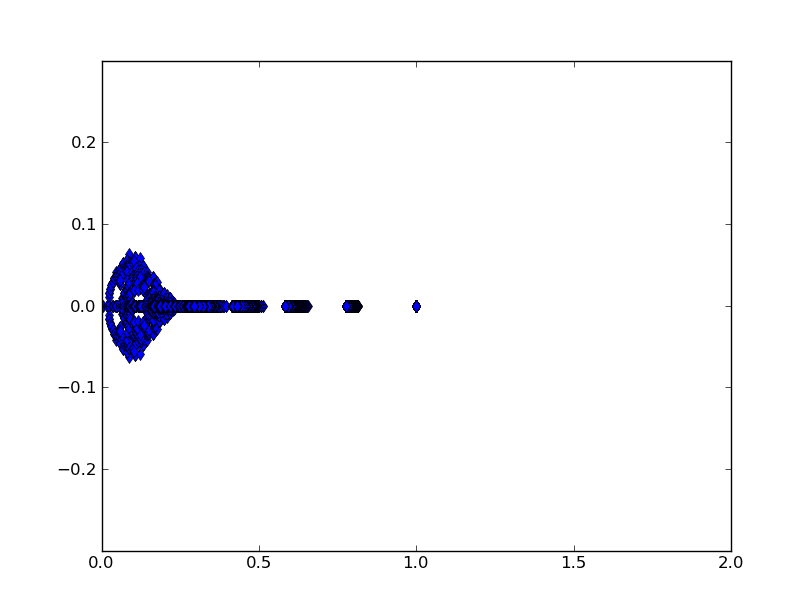
\includegraphics[width=9cm]{s8_5_5}
\caption{Spectrum of the sweep preconditioned system}
\label{fig:spectrum_sweep}
\end{figure}

\begin{figure}[H]
\centering
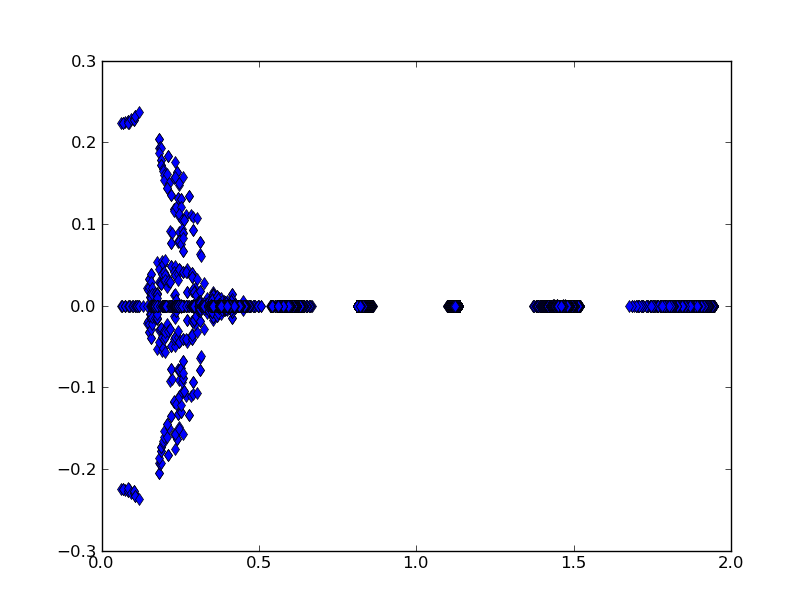
\includegraphics[width=9cm]{d_s8_5_5}
\caption{Spectrum of the DSA preconditioned system}
\label{fig:spectrum_DSA}
\end{figure}

\begin{figure}[H]
\centering
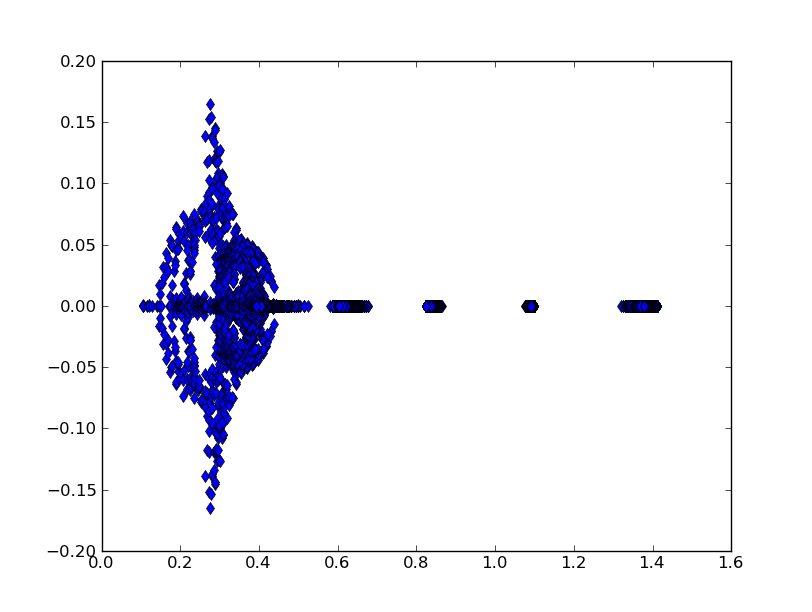
\includegraphics[width=9cm]{p_s8_5_5}
\caption{Spectrum of the Angular Multigrid with DSA preconditioned system}
\label{fig:spectrum_ANMG}
\end{figure}

On these Figures, we can note that sweep preconditioning is not effective as many eigenvalues
are located DSA moves the eigenvalues away from
zero. This explains the faster convergence of GMRES with DSA preconditioning
compared to sweep preconditioning. ANMG moves the
eigenvalues even further away than DSA and clusters them more compared to DSA.
It is obvious from these Figures that ANMG preconditioning should converge much faster than
DSA preconditioning. %which is what was observed in the previous tests. 

%-------------------------
%%%%%%%%%%%%%%%%%%%%%%%%%%%%%%%%%%%%%%%%%%%%%%%%%%%%%%%%%%%%%%%%%%%%%%%%%%%%%%%%%%%%
%%%%%%%%%%%%%%%%%%%%%%%%%%%%%%%%%%%%%%%%%%%%%%%%%%%%%%%%%%%%%%%%%%%%%%%%%%%%%%%%%%%%
\section{Results} \label{sec:results}
%%%%%%%%%%%%%%%%%%%%%%%%%%%%%%%%%%%%%%%%%%%%%%%%%%%%%%%%%%%%%%%%%%%%%%%%%%%%%%%%%%%%
%%%%%%%%%%%%%%%%%%%%%%%%%%%%%%%%%%%%%%%%%%%%%%%%%%%%%%%%%%%%%%%%%%%%%%%%%%%%%%%%%%%%

In this section, we first compare the number of GMRES iterations needed by 
ANMG-DSA and ANMG-P1SA to solve a test case problem. Then, both the number of GMRES 
iterations and the elapsed time are compared for three methods:
\begin{itemize}
\item Sweep preconditioning (S).
\item DSA with optimal transport correction preconditioning (DSA).
\item Angular multigrid with DSA preconditioning (ANMG-DSA).
\end{itemize}
The tests use a homogeneous medium and Fokker-Planck cross
sections with $\alpha=1$. $\Sigma_{t}$ is chosen to be equal to
$\Sigma_{s,0}$. The quadrature is the Gauss-Legendre-Chebyshev Galerkin
quadrature. The domain is a $5cm$ side square and the uniform mesh is composed
of 50 by 50 
cells. The GMRES solver is converged to a relative tolerance of $10^{-4}$.

%%%%%%%%%%%%%%%%%%%%%%%%%%%%%%%%%%%%%%%%%%%%%%%%%%%%%%%%%%%%%%%%%%%%%%%%%%%%%%%%%%%%
\subsection{Comparison between ANMG-DSA and ANMG-P1SA}
%%%%%%%%%%%%%%%%%%%%%%%%%%%%%%%%%%%%%%%%%%%%%%%%%%%%%%%%%%%%%%%%%%%%%%%%%%%%%%%%%%%%

The number of GMRES iterations needed to solve ANMG-DSA and
ANMG-P1SA are compared, see \tbl{tab:1}. It should be noticed that it is
harder to solve the P1SA, which positive definite, than the DSA which is
symmetric positive definite. The comparison is done for $S_4$, $S_8$ and
$S_{16}$. 
\begin{table}[H]
\begin{center}
\begin{tabular}{|c|c|c|c|c|c|}
\hline
\multicolumn{2}{|c|}{$S_4$} & \multicolumn{2}{c|}{$S_8$} &
\multicolumn{2}{c|}{$S_{16}$}\\
\hline
ANMG-DSA & ANMG-P1SA & ANMG-DSA & ANMG-P1SA & ANMG-DSA & ANMG-P1SA\\
\hline
17 &  15 & 23 & 28 & 42 & 70\\
\hline
\end{tabular}
\caption{Number of GMRES iterations to solve the test case for ANMG-DSA and
ANMG-P1SA}
\label{tab:1}
\end{center}
\end{table}
%
From \tbl{tab:1}, it can be seen than ANMG-DSA outperforms ANMG-P1SA except for
$S_4$. When the anisotropy of the problem increases, the advantage of ANMG-DSA
over ANMG-P1SA increases. For this reason, only the ANMG-DSA will be compared
to Sweep and DSA preconditioning in the next two tests.

%%%%%%%%%%%%%%%%%%%%%%%%%%%%%%%%%%%%%%%%%%%%%%%%%%%%%%%%%%%%%%%%%%%%%%%%%%%%%%%%%%%%
\subsection{Test Case with a Volumetric Source}
%%%%%%%%%%%%%%%%%%%%%%%%%%%%%%%%%%%%%%%%%%%%%%%%%%%%%%%%%%%%%%%%%%%%%%%%%%%%%%%%%%%%

For this test, there is an uniform isotropic source of intensity 10 $n/(cm^3s)$. 
We compare the results for the following quadrature order : $S_4$, $S_8$ and 
$S_{16}$. The thickness of the slab varies from
50 to 680 mean-free-path but stays constant at five transport mean-free-path.
\begin{table}[H]
\begin{center}
\begin{tabular}{|c|c|c|c|c|c|c|c|c|}
\hline
\multicolumn{3}{|c|}{$S_4$} & \multicolumn{3}{c|}{$S_8$} & 
\multicolumn{3}{c|}{$S_{16}$} \\
\hline  
S & DSA & ANMG-DSA & S & DSA & ANMG-DSA & S & DSA & ANMG-DSA\\
\hline
63 & 28 & 17 & 251 & 67 & 23 & 10840 & 175 & 42 \\
\hline
\end{tabular}
\caption{Number of GMRES iterations to solve the test problem using sweep, DSA
and ANMG-DSA preconditioning}
\tbl{tab:2}
\end{center}
\end{table}
%
%
\begin{table}[H]
\begin{center}
\begin{tabular}{|c|c|c|c|c|c|c|c|c|}
\hline
\multicolumn{3}{|c|}{$S_4$} & \multicolumn{3}{c|}{$S_8$} & 
\multicolumn{3}{c|}{$S_{16}$} \\
\hline  
S & DSA & ANMG-DSA & S & DSA & ANMG-DSA & S & DSA & ANMG-DSA\\
\hline
283 & 1067 & 667 & 4351 & 4147 & 1331 & 67948 & 17595 & 5226 \\
\hline
\end{tabular}
\caption{Elapsed time (s) to solve the test problem using sweep, DSA and
ANMG-DSA preconditioning}
\tbl{tab:3}
\end{center}
\end{table}
It can be noticed that while ANMG-DSA needs the least number of iterations to converge, it is
not always the fastest method. This is due to the work required by the extra
sweeps. However, as the anisotropy of the problem increases the advantage of
ANMG-DSA becomes obvious. For the $S_{16}$ quadrature, ANMG-DSA requires 20 times 
fewer iterations and 12 times less CPU time than sweep preconditioning. 
Compared to DSA, ANMG-DSA needs four times fewer iterations and three times less 
time. It is interesting to note that DSA is never more efficient (in elapsed
time and number of iterations) than ANMG-DSA.

%%%%%%%%%%%%%%%%%%%%%%%%%%%%%%%%%%%%%%%%%%%%%%%%%%%%%%%%%%%%%%%%%%%%%%%%%%%%%%%%%%%%
\subsection{Test Case with a Boundary Source (Beam problem)}
%%%%%%%%%%%%%%%%%%%%%%%%%%%%%%%%%%%%%%%%%%%%%%%%%%%%%%%%%%%%%%%%%%%%%%%%%%%%%%%%%%%%

Now, we compare the number of GMRES iterations and the time needed to solve a
beam problem. We use a $S_8$ quadrature and there is an incoming flux coming
from the left for $y\in [2cm,3cm]$ of intensity 10 $n/(cm^3s)$. The flux is
coming from the most normal directions of the quadrature.
\begin{table}[H]
\begin{center}
\begin{tabular}{|c|c|c|}
\hline
S & DSA & ANMG-DSA\\
\hline
235 & 60 & 26 \\
\hline
\end{tabular}
\caption{GMRES iterations to solve the test problem using sweep, DSA and
ANMG-DSA preconditioning}
\tbl{tab:4}
\end{center}
\end{table}

\begin{table}[H]
\begin{center}
\begin{tabular}{|c|c|c|}
\hline
S & DSA & ANMG-DSA\\
\hline
3855 & 2287 & 1227\\
\hline
\end{tabular}
\caption{Elapsed time (s) to solve the test problem using sweep, DSA and
ANMG-DSA preconditioning}
\tbl{tab:5}
\end{center}
\end{table}
%
These results confirm the previous ones and show the advantage of the angular
multigrid preconditioning over the DSA preconditioning.

%-------------------------
%%%%%%%%%%%%%%%%%%%%%%%%%%%%%%%%%%%%%%%%%%%%%%%%%%%%%%%%%%%%%%%%%%%%%%%%%%%%%%%%%%%%
%%%%%%%%%%%%%%%%%%%%%%%%%%%%%%%%%%%%%%%%%%%%%%%%%%%%%%%%%%%%%%%%%%%%%%%%%%%%%%%%%%%%
\section{Conclusions} \label{sec:conclusions}
%%%%%%%%%%%%%%%%%%%%%%%%%%%%%%%%%%%%%%%%%%%%%%%%%%%%%%%%%%%%%%%%%%%%%%%%%%%%%%%%%%%%
%%%%%%%%%%%%%%%%%%%%%%%%%%%%%%%%%%%%%%%%%%%%%%%%%%%%%%%%%%%%%%%%%%%%%%%%%%%%%%%%%%%%

In this paper, we have recalled previous work on the angular multigrid
method (ANMG) applied to the $S_n$ equations for highly forward peaked scattering problems. 
For one dimensional geometry, this scheme has been proven to be very 
efficient compared to DSA preconditioning. When using Fokker-Planck cross sections, the
spectral radius of the method is bounded by 0.6 while SI+DSA is bounded by 1. 
For multidimensional problems, the generalization of the ANMG scheme to multi-dimensions (the
PAMNF and PAMF methods) does not exhibit the same behavior. To remain stable, the angular 
multigrid method needs to be stabilized
by a filter which degrades the spectral radius (PAMF method). The spectral radius is smaller 
to the one from  DSA preconditioning but it can still be arbitrary close to one. 

Unlike the previous ANMG methods which solved the $S_n$ equations using  Source 
Iteration, we recast the angular multigrid method as a preconditioner 
for Krylov solvers. Two variants, which differ at the coarsest angular level,
have been tested. One uses the sequence $S_n,S_{\lceil\frac{n}{2}\rceil},
\hdots,S_4,P1SA$, while the other uses the sequence $S_n,
S_{\lceil\frac{n}{2}\rceil},\hdots,S_2,DSA$.
The first sequence was proposed in \cite{multigrid_1d}, the second in 
\cite{multigrid_2d}. In \cite{multigrid_2d}, the authors did not use the first
sequence because it is known to be unstable for multidimensional problem when 
solved  using SI. Here, both sequences were solved using GMRES as Krylov solver; 
both were found to give satisfactory results and the second sequence was shown to be more 
efficient, i.e., the number of GMRES iterations is smaller for highly 
anisotropic medium and P1SA (PD) is more difficult to invert than
DSA (SPD). The number of GMRES iterations and the time needed
to solve the equations were compared for sweep preconditioning, DSA
preconditioning and angular multigrid-DSA preconditioning. The angular
multigrid was shown to be always faster and needed fewer iterations than DSA.
For highly anisotropic scattering, GMRES with angular multigrid
preconditioning is much faster than GMRES with DSA or sweep preconditioning.
The comparison of the eigenvalue spectrum of the three methods shows that 
DSA preconditioner moves the eigenvalues away from zero. The new
preconditioner moves the eigenvalues further away from zero and keeps them
closer to each others compare to DSA. This explains the
efficiency of the angular multigrid method used as a preconditioner for Krylov solvers.


%%%%%%%%%%%%%%%%%%%%%%%%%%%%%%%%%%%%%%%%%%%%%%%%%%%%%%%%%%%%%%%%%%%%

\bibliographystyle{unsrt}
\bibliography{biblio}

%%%%%%%%%%%%%%%%%%%%%%%%%%%%%%%%%%%%%%%%%%%%%%%%%%%%%%%%%%%%%%%%%%%%
%%%%%%%%%%%%%%%%%%%%%%%%%%%%%%%%%%%%%%%%%%%%%%%%%%%%%%%%%%%%%%%%%%%%
%-------------------------
%%%%%%%%%%%%%%%%%%%%%%%%%%%%%%%%%%%%%%%%%%%%%%%%%%%%%%%%%%%%%%%%%%%%%%%%%%%%%%%%%%%%
%%%%%%%%%%%%%%%%%%%%%%%%%%%%%%%%%%%%%%%%%%%%%%%%%%%%%%%%%%%%%%%%%%%%%%%%%%%%%%%%%%%%
\begin{appendices}
\section{Appendix}
\subsection{MIP-DSA}
We will recall here the weak form of the MIP-DSA \cite{mip} :
\begin{equation}
b_{MIP}(\phi,\phi^*) = l_{MIP}(\phi^*)
\end{equation}
with :
\begin{equation}
\begin{split}
b_{MIP}(\phi,\phi^*) =& (\Sigma_a \phi,\phi^*)_{\partial D} +
\(\mathrm{D}\bn\phi,\bn\phi^*\)_{\mathcal{D}} + \(\kappa_e\llb\phi\rrb,
\llb\phi^*\rrb\)_{E_h^i}
+ \(\llb\phi\rrb,\ldb \mathrm{D}\partial_n \phi^*\rdb\)_{E_h^i} +\\
&(\ldb \mathrm{D} \partial_n \phi\rdb,\llb\phi^*\rrb)_{E_h^i} + 
(\kappa_e\phi,\phi^*)_{\partial
D^d}-\frac{1}{2} \(\phi,\mathrm{D}\partial_n \phi^*\)_{\partial
\mathcal{D}^d} - \frac{1}{2} (\mathrm{D} \partial_n \phi,\phi^*)_{\partial 
\mathcal{D}^d}
\end{split}
\end{equation}
\begin{equation}
l_{MIP}(\phi^*) = (Q_0,\phi^*)_{\mathcal{D}} 
\end{equation}
where :
\begin{itemize}
\item $(f,g)_{\mathcal{D}} = \sum_{K\in \mathbb{T}_h} \int_K fg\ d\br$ and 
$(f,g)_{E_h^i} = \sum_{e\in E_h^i} \int_e fg\ ds$
\item $\mathbb{T}_h$ is the mesh used to discretize the domain $\mathcal{D}$
into nonoverlapping elements $K$, $E_h^i$ is the set of interior edges,
$\mathcal{D}$ is the spatial domain, $\partial \mathcal{D}^d$ is the boundary
of the domain with Dirichlet condition and $\partial \mathcal{D}^r$ is the
boundary of the domain with reflective condition
\item $\Sigma_a$ is the absorption macroscopic cross section
\item $\mathrm{D}$ is the diffusion coefficient
\item $\partial_n = \bs{n}\cdot \bn$ where $\bs{n}$ is the outward unit
normal
\item $\llb \phi\rrb = \phi^{+}-\phi^{-}$ is the jump of at the interface
between two elements
\item $\ldb\phi\rdb = \frac{\phi^++\phi^-}{2}$ is the mean of $\phi$ at the
interface between two elements
\item $\phi^{\pm}(\br)=\lim_{s\to 0^{\pm}}\phi(\br+s\bs{n}_e)$, $\bs{n}_e$ is
the normal unit vector associated with a given edge $e$
\item $\kappa_e = \max\(\kappa_e^{IP},\frac{1}{4}\)$ with
$\kappa_e^{IP}=\left\{
\begin{aligned}
&\frac{c(p^+)}{2}\frac{D^+}{h_{\bot}^+} + \frac{c(p^-)}{2}
\frac{D^-}{h_{\bot}^-} &\textrm{ on interior edges, i.e. }e\in E_h^i\\
&c(p)\frac{D}{h_{\bot}} & \textrm{ on boundary edges,
i.e. }e\in\partial\mathcal{D}^d
\end{aligned}
\right.$\\
$c(p)$ is given by $c(p)=2p(p+1)$, $p$ is the polynomial order and $h_{\bot}$
is the length of the cell in the direction orthogonal to the edge $e$
\end{itemize}
\subsection{P1C}
The P1C scheme, which is positive definite but non-symmetric, is given by :
\begin{equation}
b_{P1C}(\Phi,\bs{J},\Phi^*,\bs{J}^*) = l_{P1C}(\Phi^*,\bs{J}^*)
\end{equation}
with :
\begin{equation}
\begin{split}
b_{P1}(\Phi,\bs{J},\Phi^*,\bs{J}^*) = & (\Sigma_a \Phi,\Phi^*)_{\mathcal{D}} +
(3\Sigma_{tr} \bs{J},\bs{J}^*)_{\mathcal{D}} + (\bn
\Phi,\bs{J}^*)_{\mathcal{D}} - (\bs{J},\bn \Phi^*)_{\mathcal{D}}\\
&+\frac{1}{4} \(\llb\Phi\rrb,\llb\Phi^*\rrb\)_{E_h^i} +
\(\llb\Phi\rrb,\ldb\bs{J}\cdot\bs{n}_e\rdb\)_{E_h^i} - (\ldb
\bs{J}\cdot\bs{n}_e\rdb, \llb\Phi^*\rrb)_{E_h^i}\\
&+\frac{9}{16}\(\llb\bs{J}\cdot\bs{n}_e\rrb,\llb\bs{J}^*\cdot\bs{n}_e\rrb\)_{E_h^i}
+ \frac{9}{16}\(\llb\bs{J}\rrb,\llb\bs{J}^*\rrb\)_{E_h^i}\\
&+\frac{1}{4}(\Phi,\Phi^*)_{\partial \mathcal{D}^d} +
\frac{1}{2}(\Phi,\bs{J}^*\cdot\bs{n}_e)_{\partial \mathcal{D}^d} - \frac{1}{2}
(\bs{J}\cdot\bs{n}_e,\Phi^*)_{\partial\mathcal{D}^d}\\
&+\frac{9}{16}(\bs{J},\bs{J}^*)_{\partial
\mathcal{D}^d}+\frac{9}{16}(\bs{J}\cdot\bs{n}_e,\bs{J}^*\cdot\bs{n}_e)_{\partial 
\mathcal{D}^d} + \frac{9}{4} (\bs{J}\cdot\bs{n}_e,\bs{J}^*\cdot\bs{n}_e)_{\partial
\mathcal{D}^r}
\end{split}
\end{equation}
\begin{equation}
l(\Phi^*,\bs{J}^*) = (Q_0,\Phi^*)_{\mathcal{D}} +
(3\bs{Q}_1,\bs{J}^*)_{\mathcal{D}}
\end{equation}
where $\bs{J}$ is the current or first moment of the flux and 
$\Sigma_{tr}=\Sigma_t-\Sigma_{s,1}$.
\end{appendices}
%%%%%%%%%%%%%%%%%%%%%%%%%%%%%%%%%%%%%%%%%%%%%%%%%%%%%%%%%%%%%%%%%%%%%%%%%%%%%%%%%%%%
%%%%%%%%%%%%%%%%%%%%%%%%%%%%%%%%%%%%%%%%%%%%%%%%%%%%%%%%%%%%%%%%%%%%%%%%%%%%%%%%%%%%

\end{document}

